\documentclass[letterpaper,12pt]{article}
\usepackage{tabularx,amsmath,graphicx}
\usepackage[margin=1in,letterpaper]{geometry}
\usepackage{cite}
\usepackage[final]{hyperref}
\hypersetup{
colorlinks=true,
linkcolor=blue,
citecolor=blue,
filecolor=magenta,
urlcolor=blue         
}
\begin{document}
\title{Lab 1: Prelab}
\author{Joshua Emele $<$jemele@acm.org$>$}
\maketitle

\section{Theory Problems}

\subsection{Spectrum of AM modulated signals}
\begin{figure}[ht] 
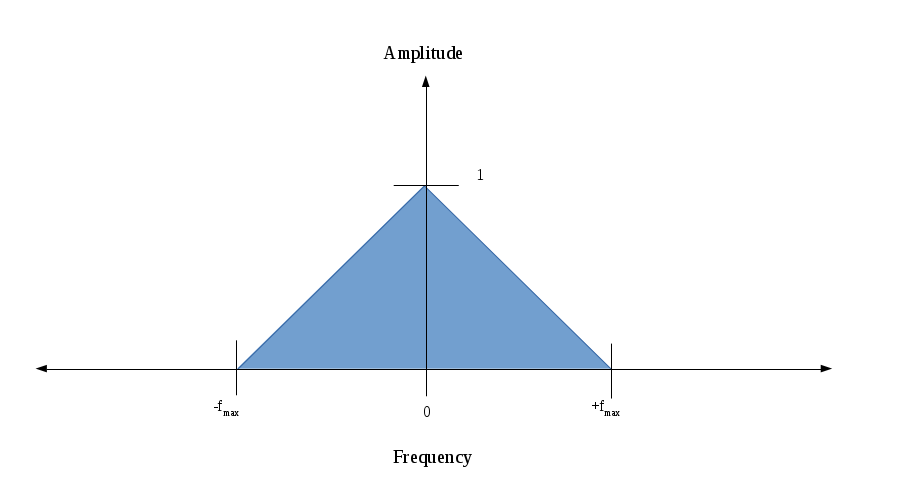
\includegraphics[width=1.0\columnwidth]{prelab1-figure1}
\caption{
\label{fig:hw1-figure1}
{\bf Describe figure 1...
here}
}
\end{figure}

\begin{figure}[ht] 
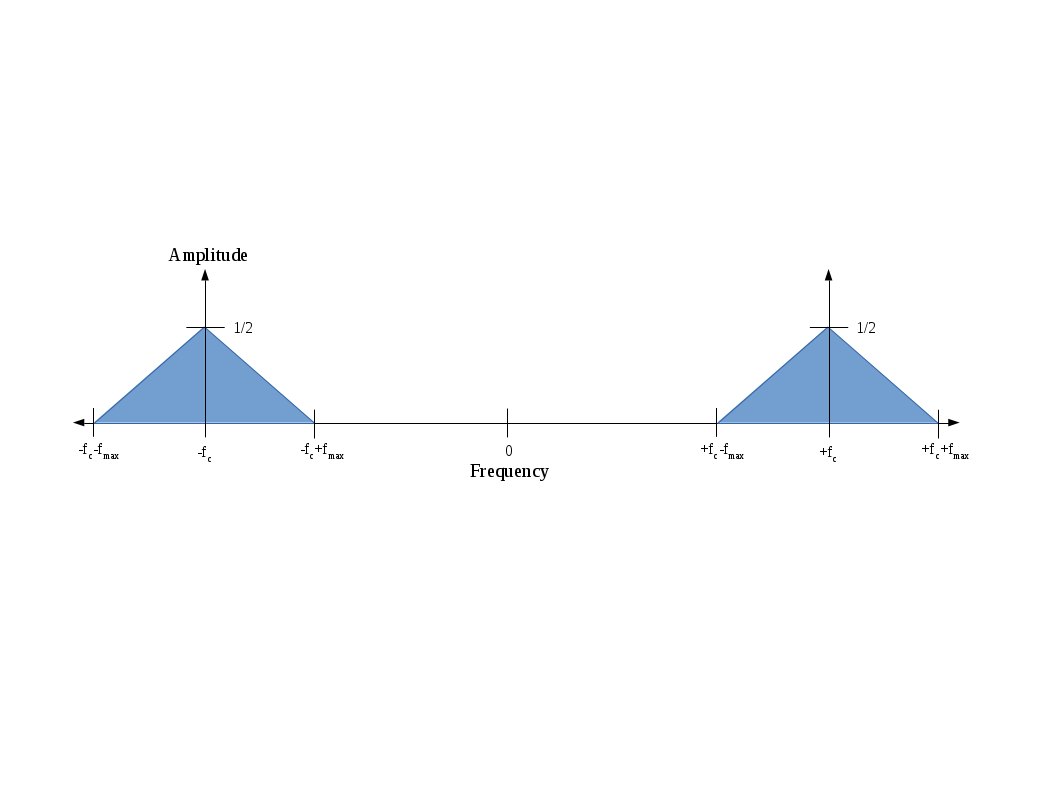
\includegraphics[width=1.0\columnwidth]{prelab1-figure1a}
\caption{
\label{fig:hw1-figure1a}
{\bf Describe figure 1a...
here}
}
\end{figure}

\begin{figure}[ht] 
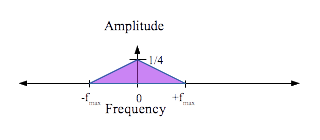
\includegraphics[width=1.0\columnwidth]{prelab1-figure1b}
\caption{
\label{fig:hw1-figure1b}
{\bf Describe figure 1b...
here}
}
\end{figure}

\subsection{Frequency demodulation errors}
\begin{figure}[ht] 
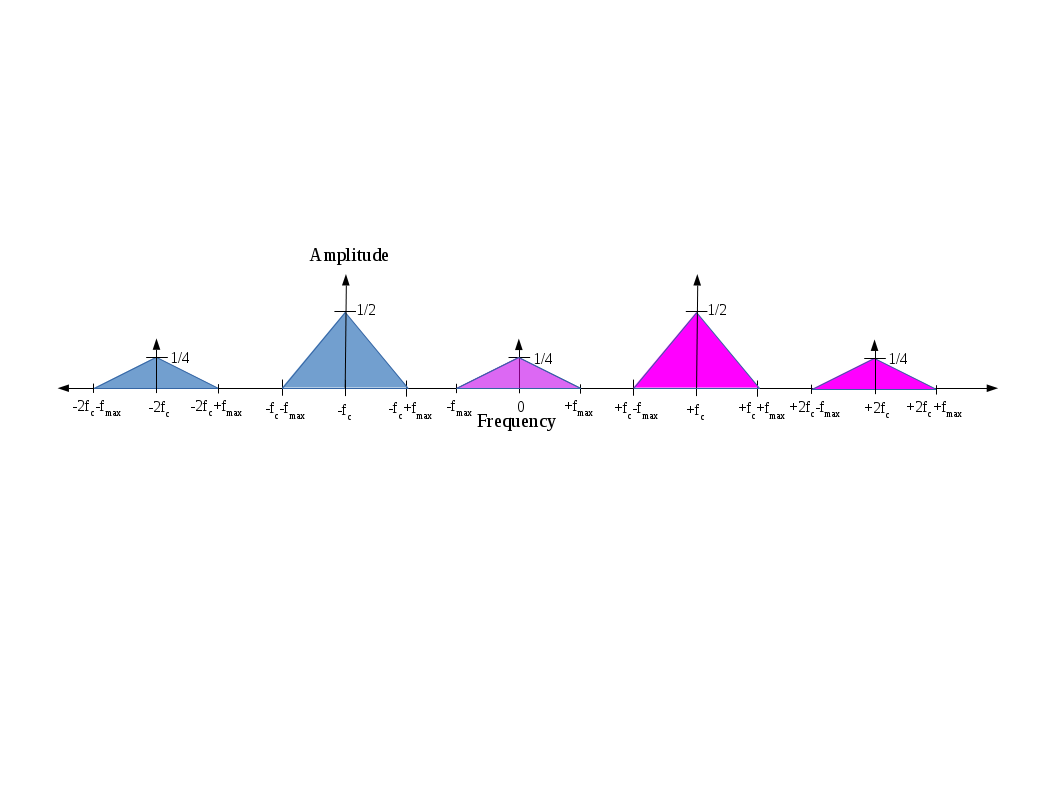
\includegraphics[width=1.0\columnwidth]{prelab1-figure2a}
\caption{
\label{fig:hw1-figure2a}
{\bf Describe  figure 2a...
here}
}
\end{figure}

\begin{figure}[ht] 
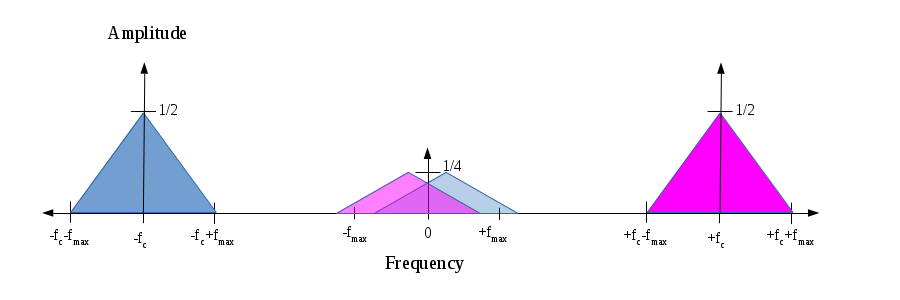
\includegraphics[width=1.0\columnwidth]{prelab1-figure2b}
\caption{
\label{fig:hw1-figure2b}
{\bf Describe  figure 2b...
here}
}
\end{figure}

\begin{figure}[ht] 
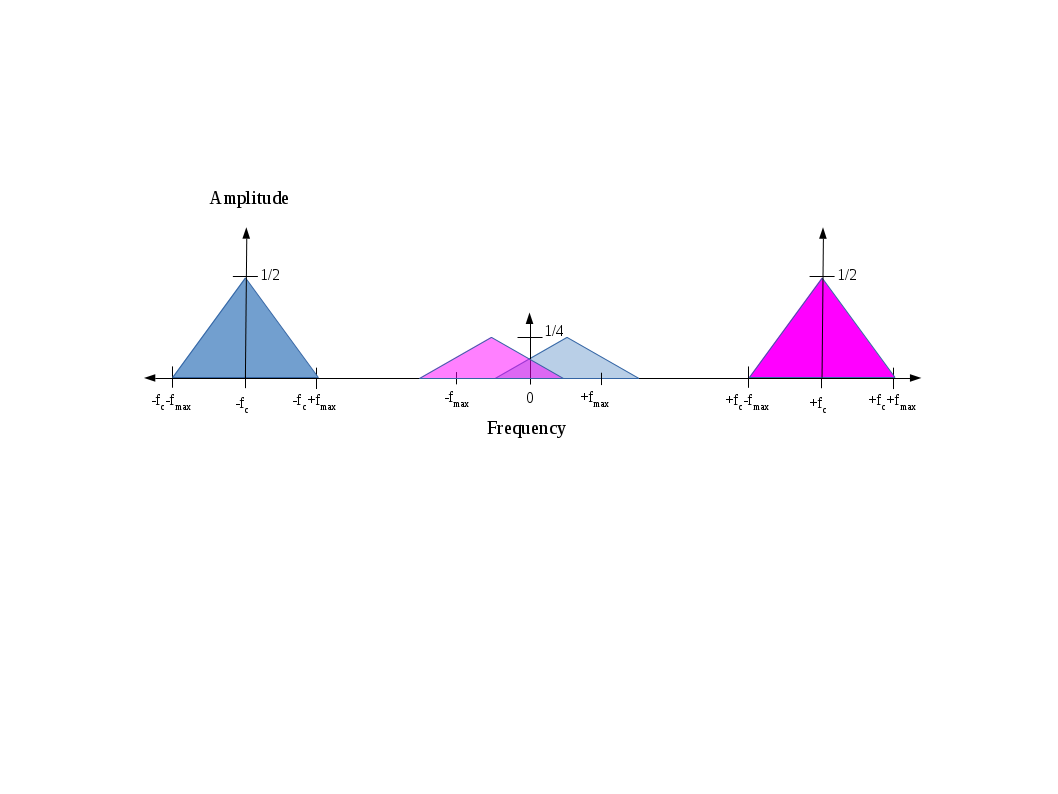
\includegraphics[width=1.0\columnwidth]{prelab1-figure2c}
\caption{
\label{fig:hw1-figure2c}
{\bf Describe  figure 2c...
here}
}
\end{figure}

\subsection{Phase demodulation errors}

An AM signal $\tilde{s}(t)=A\ cos(2 \pi f_{c}t)$ where $A$ is a constant is
demodulated by $cos(2 \pi f_{c}t+\phi)$ where $\phi$ represents a phase error.

An expression for the demodulated signal $d(t,\phi)$ as a function of the phase
error $\phi$ is given by:
\begin{equation}
d(t,\phi)=A\ cos(2 \pi f_{c}t)cos(2 \pi f_{c}t+\phi)
\end{equation}

The period of the carrier $f_{c}$ is given by $T=\frac{1}{f_{c}}$.

If the demodulated signal $d(t,\phi)$ is integrated over a time period $T$ that
is many times the period of the carrier (i.e., $N\ T$, where $N >= 2$), the value
of the integral without phase error ($\phi=0$) is given by:

\begin{equation}
\begin{split}
M_{0} & = \int_{0}^{\frac{2}{f}}A\ cos(2\pi f_{c}t)cos(2\pi f_{c}t) \\
 & = \frac{1}{f}
\end{split}
\end{equation}

The value of the integral with phase error ($\phi\neq0$) over the same period is
given by:

\begin{equation}
\begin{split}
M_{1} & = \int_{0}^{\frac{2}{f}}A\ cos(2\pi f_{c}t)cos(2\pi f_{c}t+\phi) \\
 & = \frac{cos(\phi)}{f}
\end{split}
\end{equation}

The maximum phase error $\phi$ that can be tolerated for the demodulated signal
to ensure the amplitude is within ten percent of the amplitude without a phase
error is given by:

\begin{equation}
\begin{split}
\frac{M_{0}}{M_{1}}\leq10 \\
sec(\phi)\leq10 \\
|\phi|\leq\ sec^{-1}(10) \\
|\phi|\leq\ 0.4706 \\
\end{split}
\end{equation}

\section{Matlab/Simulink Simulations}

\end{document}
